
%----------------------------------------------------------------------------------------
%	Lecture 3
%----------------------------------------------------------------------------------------

\chapter{Key concepts in quantum mechanic}

\bigbreak
\section{The Wavefunction}

The Wavefunction is usually denoted by the symbol $\Psi$. 
It is a function of space and time, that is, $\Psi(x, y, z, t)$
The key fact here is that $\Psi$ is a complex function, that is, 
the value of $\Psi$ at any point is a complex number.

Although $\Psi$ represents the state of the system, 
it doesn't give you the position of the particles.
It only gives you probabbilities.

What is physically meaningful is the squared magnitute of $\Psi$, that is, 
$|\Psi|^2$ is realted to the probability of finding the system in any particular state.

\section{Operators}

Operators connect the Wavefunction to the observables that we can measure.
They are denoted by letters with hats, i.e., $\hat{x}, \hat{p}$.
The Operators act on the Wavefunction : $\hat{x} \Psi$ and $\hat{p} \Psi$.

Now, $\hat{x}$ can be thought of as just multiplying by $x$. 
So $\hat{x} \Psi(x) = x \cdot \Psi(x)$.
Now, $\hat{p} = - \hbar \px{}{x}$.
Note that $\hat{p} \Psi$ is not momentum of $\Psi$.

\section{Schrodinger's Equation}

$\hat{H}$ is the Hamiltonian Operator which is same as the energy.
So it can be writter down as sum of kinetic energy operator and potential energy operator.

$$ 
i \hbar \px{\Psi}{t} 
    = \hat{H} \Psi 
    = (\hat{KE} + \hat{V}) \Psi 
    = - \frac{\hbar^2}{2m} \pxx{\Psi}{x} + V(x) \Psi
$$

Most QM we'll be seeing is solving this equation for particular systems.


\begin{figure}[ht!]
	\centering
	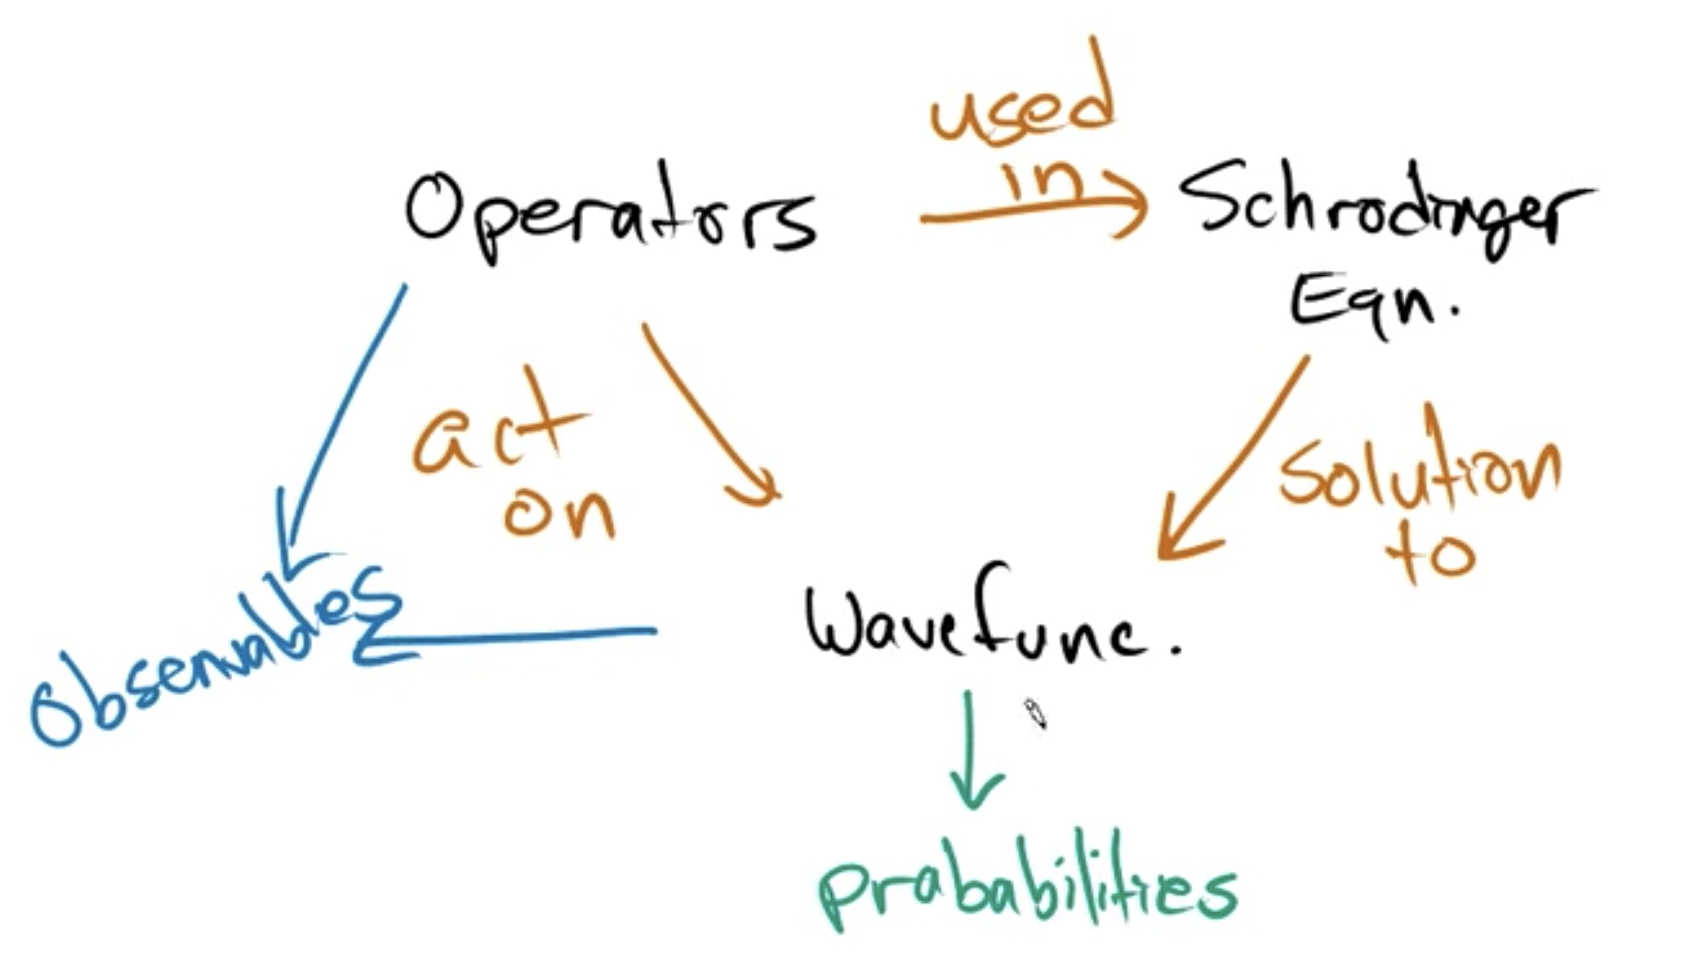
\includegraphics[scale=0.3]{./images/lecture_3_figure_1.png}
	\caption{Map of QM}
\end{figure}